%%%%%%%%%%%%%%%%%%%%%%%%%%%%%%%%%%%%%%%%%%%%%%%%%%%%%%%%%%%%%%%%%%%%%
%
% CS484 Written Question Template
%
% This is a LaTeX document. LaTeX is a markup language for producing 
% documents. Your task is to fill out this document, then to compile 
% it into a PDF document. 
%
% 
% TO COMPILE:
% > pdflatex thisfile.tex
%
% If you do not have LaTeX and need a LaTeX distribution:
% - Personal laptops (all common OS): www.latex-project.org/get/
% - We recommend miktex (https://miktex.org/) for latex engine,
%   and TeXstudio(http://www.texstudio.org/) for latex editor.
%   You should install both programs for editing latex.
%   Or you can use Overleaf (https://www.overleaf.com/) which is 
%   an online latex editor.
%
% If you need help with LaTeX, please come to office hours. 
% Or, there is plenty of help online:
% https://en.wikibooks.org/wiki/LaTeX
%
% Good luck!
% Min and the CS484 staff
%
%%%%%%%%%%%%%%%%%%%%%%%%%%%%%%%%%%%%%%%%%%%%%%%%%%%%%%%%%%%%%%%%%%%%%

\documentclass[11pt]{article}

\usepackage[english]{babel}
\usepackage[utf8]{inputenc}
\usepackage[colorlinks = true,
            linkcolor = blue,
            urlcolor  = blue]{hyperref}
\usepackage[a4paper,margin=1.5in]{geometry}
\usepackage{stackengine,graphicx}
\usepackage{fancyhdr}
\setlength{\headheight}{15pt}
\usepackage{microtype}
\usepackage{times}

\usepackage{graphicx}
\DeclareGraphicsExtensions{.pdf,.png,.jpg}


% From https://ctan.org/pkg/matlab-prettifier
\usepackage[numbered,framed]{matlab-prettifier}

\frenchspacing
\setlength{\parindent}{0cm} % Default is 15pt.
\setlength{\parskip}{0.3cm plus1mm minus1mm}

\pagestyle{fancy}
\fancyhf{}
\lhead{Homework 1 Questions}
\rhead{CS484}
\rfoot{\thepage}

\date{}

\title{\vspace{-1cm}Homework 1 Questions}


\begin{document}
\maketitle
\vspace{-2cm}
\thispagestyle{fancy}

\section*{Instructions}
\begin{itemize}
  \item Compile and read through the included MATLAB tutorial.
  \item 2 questions.
  \item Include code.
  \item Feel free to include images or equations.
  \item Please make this document anonymous.
  \item \textbf{Please use only the space provided and keep the page breaks.} Please do not make new pages, nor remove pages. The document is a template to help grading.
  \item If you really need extra space, please use new pages at the end of the document and refer us to it in your answers.
\end{itemize}


\section*{Submission}
\begin{itemize}
	\item Please zip your folder with \textbf{hw1\_student id\_name.zip} $($ex: hw1\_20181234\_Peter.zip$)$
	\item Submit your homework to \href{http://klms.kaist.ac.kr/course/view.php?id=99418}{KLMS}.
	\item An assignment after its original due date will be degraded from the marked credit per day: e.g., A will be downgraded to B for one-day delayed submission.
\end{itemize}

\pagebreak


\section*{Questions}


%%%%%%%%%%%%%%%%%%%%%%%%%%%%%%%%%%%

% Please leave the pagebreak
\paragraph{Q1:} We wish to set all pixels that have a brightness of 10 or less to 0, to remove sensor noise. However, our code is slow when run on a database with 1000 grayscale images.

\emph{Image:} \href{grizzlypeakg.png}{grizzlypeakg.png}

\begin{lstlisting}[style=Matlab-editor]
A = imread('grizzlypeakg.png');
[m1,n1] = size( A );
for i=1:m1
    for j=1:n1
        if A(i,j) <= 10
            A(i,j) = 0;
        end
    end
end
\end{lstlisting}

\paragraph{Q1.1:} How could we speed it up?

%%%%%%%%%%%%%%%%%%%%%%%%%%%%%%%%%%%
\paragraph{A1.1:} Your answer here.

\begin{lstlisting}[style=Matlab-editor]
B=imread('grizzlypeakg.png');
[m2,n2] = size( B );
C = B < 10;
B(C) = 0;
\end{lstlisting}

%%%%%%%%%%%%%%%%%%%%%%%%%%%%%%%%%%%

% Please leave the pagebreak
\pagebreak
\paragraph{Q1.2:} What factor speedup would we receive over 1000 images? Please measure it.

Ignore file loading; assume all images are equal resolution; don't assume that the time taken for one image $\times1000$ will equal $1000$ image computations, as single short tasks on multitasking computers often take variable time.

%%%%%%%%%%%%%%%%%%%%%%%%%%%%%%%%%%%
\paragraph{A1.2:} Your answer here.
\begin{lstlisting}[style=Matlab-editor]
tic
for k=0:999
    A=imread('grizzlypeakg.png');
    [m1,n1] = size( A );
    for i=1:m1
        for j=1:n1
            if A(i,j)<=10
                A(i,j) = 0;
            end
        end
    end
    A=zeros(m1,n1);
end
fprintf('method 1:');
toc

tic
for k=0:999
    B=imread('grizzlypeakg.png');
    [m2,n2] = size( B );
    C = B <= 10;
    B(C) = 0;
    B=zeros(m2,n2);
end
fprintf('method 2:');
toc
\end{lstlisting}
\begin{verbatim}
>> CV1_2
method 1:Elapsed time is 38.371711 seconds.
method 2:Elapsed time is 29.715092 seconds.
\end{verbatim}

%%%%%%%%%%%%%%%%%%%%%%%%%%%%%%%%%%%

% Please leave the pagebreak
\pagebreak
\paragraph{Q1.3:} How might a speeded-up version change for color images? Please measure it.

\emph{Image:} \href{grizzlypeak.jpg}{grizzlypeak.jpg}

%%%%%%%%%%%%%%%%%%%%%%%%%%%%%%%%%%%
\paragraph{A1.3:} Your answer here.

\begin{figure}[h]

\centering

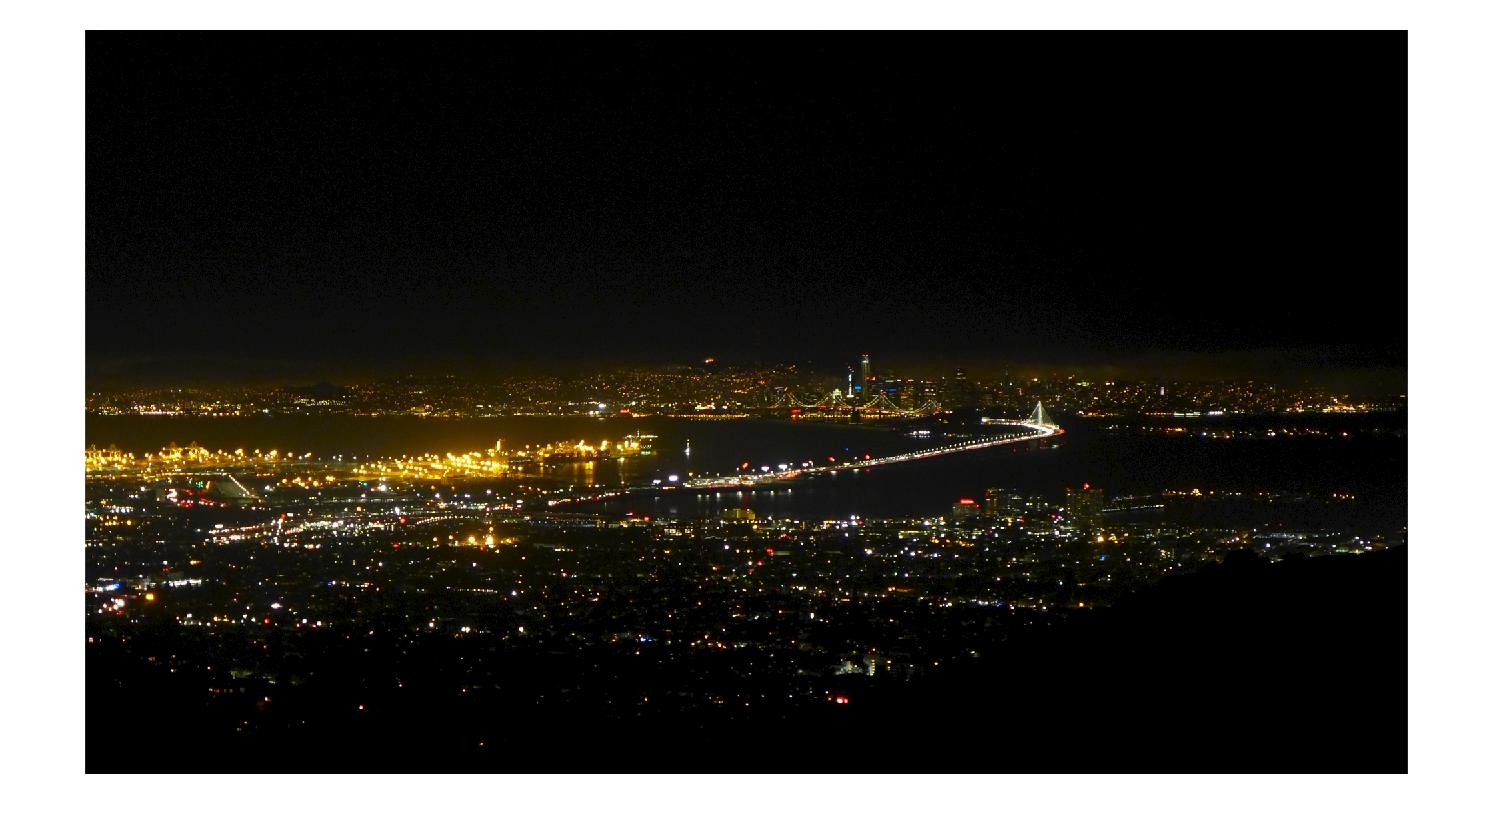
\includegraphics[width=1\textwidth]{P1_3.jpg}

\end{figure}

\begin{verbatim}
>> CV1_3
1 try, method 1:Elapsed time is 6.063604 seconds.
1 try, method 2:Elapsed time is 0.034056 seconds.
2 try, method 1:Elapsed time is 6.077723 seconds.
2 try, method 2:Elapsed time is 0.035354 seconds.
3 try, method 1:Elapsed time is 6.229049 seconds.
3 try, method 2:Elapsed time is 0.036830 seconds.
4 try, method 1:Elapsed time is 6.051567 seconds.
4 try, method 2:Elapsed time is 0.037339 seconds.
5 try, method 1:Elapsed time is 5.995840 seconds.
5 try, method 2:Elapsed time is 0.035910 seconds.
6 try, method 1:Elapsed time is 6.090698 seconds.
6 try, method 2:Elapsed time is 0.034144 seconds.
7 try, method 1:Elapsed time is 5.853549 seconds.
7 try, method 2:Elapsed time is 0.034807 seconds.
8 try, method 1:Elapsed time is 5.905430 seconds.
8 try, method 2:Elapsed time is 0.033173 seconds.
9 try, method 1:Elapsed time is 6.270601 seconds.
9 try, method 2:Elapsed time is 0.034299 seconds.
10 try, method 1:Elapsed time is 5.843067 seconds.
10 try, method 2:Elapsed time is 0.034772 seconds.
\end{verbatim}
%%%%%%%%%%%%%%%%%%%%%%%%%%%%%%%%%%%

% Please leave the pagebreak
\pagebreak
\paragraph{Q2:} We wish to reduce the brightness of an image but, when trying to visualize the result, all we sees is white with some weird ``corruption'' of color patches.

\emph{Image:} \href{gigi.jpg}{gigi.jpg}

\begin{lstlisting}[style=Matlab-editor]
I = double( imread('gigi.jpg') );
I = I - 20;
imshow( I );
\end{lstlisting}

\paragraph{Q2.1:} What is incorrect with this approach? How can it be fixed while maintaining the same amount of brightness reduction?

%%%%%%%%%%%%%%%%%%%%%%%%%%%%%%%%%%%
\paragraph{A2.1:} Your answer here.

I should use im2double instead of double function.
\begin{lstlisting}[style=Matlab-editor]
I = imread('gigi.jpg');
I = I - 20;
doubleI = im2double(I);
imshow(doubleI);
\end{lstlisting}



%%%%%%%%%%%%%%%%%%%%%%%%%%%%%%%%%%%

% Please leave the pagebreak
\pagebreak
\paragraph{Q2.2:} Where did the original corruption come from? Which specific values in the original image did it represent?

%%%%%%%%%%%%%%%%%%%%%%%%%%%%%%%%%%%
\paragraph{A2.2:} Your answer here.

\begin{lstlisting}[style=Matlab-editor]
I1 = im2double(imread('gigi.jpg'));
I1 = I1 - 20;

I2 = imread('gigi.jpg');
I2 = I2 - 20;
doubleI2 = double(I2);
\end{lstlisting}
In code, I1 and doubleI2 are both problematic.

	If you use "im2double" function, the value of (uint8) 0-255 changes to (double) 0-1.  I1 used an "im2double" function, but after using the function, it did -20. So all black out. I2 did -20 first, but not im2double function. So It makes "corruption". 



%%%%%%%%%%%%%%%%%%%%%%%%%%%%%%%%%%%

\end{document}